% !TEX root = ../eval.tex

\section{Results}%
\label{sec:results}


\subsection{Main results}%
\label{sub:main_results}

\begin{itemize}

    \item Figure~\ref{fig:main_results} shows the effect of app use on monthly
        discretionary spend (top row) and monthly net-inflows into savings
        accounts (bottom row) under the unconditional (left column) and
        conditional (right column) parallel trends assumptions.

    \item Estimates are group-time average treatment effects aggregated by time
        since treatment exposure.

    \item All results are presented with a uniform 95\% confidence band, based
        on bootstrapped standard errors clustered at the user level that also
        account for autocorrelation in the data.\footnote{A uniform 95\%
            confidence band accounts for multiple hypothesis testing in that it
            is constructed such that \textit{all} shown coefficients cover
            their corresponding true value 95 percent of the time. In contrast,
            a more commonly used pointwise 95\% confidence band is constructed
        such that the confidence interval for each parameter covers the true
    parameter 95 percent of the time.}

    \item Conditional results use the doubly-robust estimator discussed in the
        methods section.

    \item We can see that discretionary spend falls by between \pounds100 and
        \pounds150 per month once users start using the app, depending on the
        parallel trends assumption used. Given that average
        monthly discretionary spend is about \pounds860 (see
        Table~\ref{tab:sumstats}), this corresponds to a drop in discretionary
        spend of about 11-17 percent, which is substantial.

    \item As discussed in Section~\ref{sub:estimation}, the conditional
        parallel trend assumption leads to different results from the
        unconditional version if (1) the paths of the outcome variables are
        parallel only for groups with similar covariate values and (2) the
        distribution of covariate values differs between treated and comparison
        group. Given that our comparison group is the set of
        ``not-yet-treated`` users rather than a set of ``never-treated`` users,
        the relatively small difference in results is as expected.

    \item At the same time, we would have expected there to be some difference.
        If we discretionary spend is a constant fraction of income and total
        spend, then we would expect parallel trends to hold only for groups
        with the same income and total monthly spend. Similarly, if we think
        that the average spend per account observed is constant, then parallel
        trends hold only for users with the same number of observed accounts
        (if we think of active accounts as observed accounts).

    \item In contrast to discretionary spend, net-inflows into savings accounts
        do not change once users start using the app. The wide confidence
        bands reflect the large variation in net-inflows already seen in
        Table~\ref{tab:sumstats}.

    \item Results indicate that parallel trend assumption might not hold. So we
        should interpret these result with some caution.

\end{itemize}


\begin{figure}[H]
    \centering 
    \caption{Main results}
    \label{fig:main_results}
    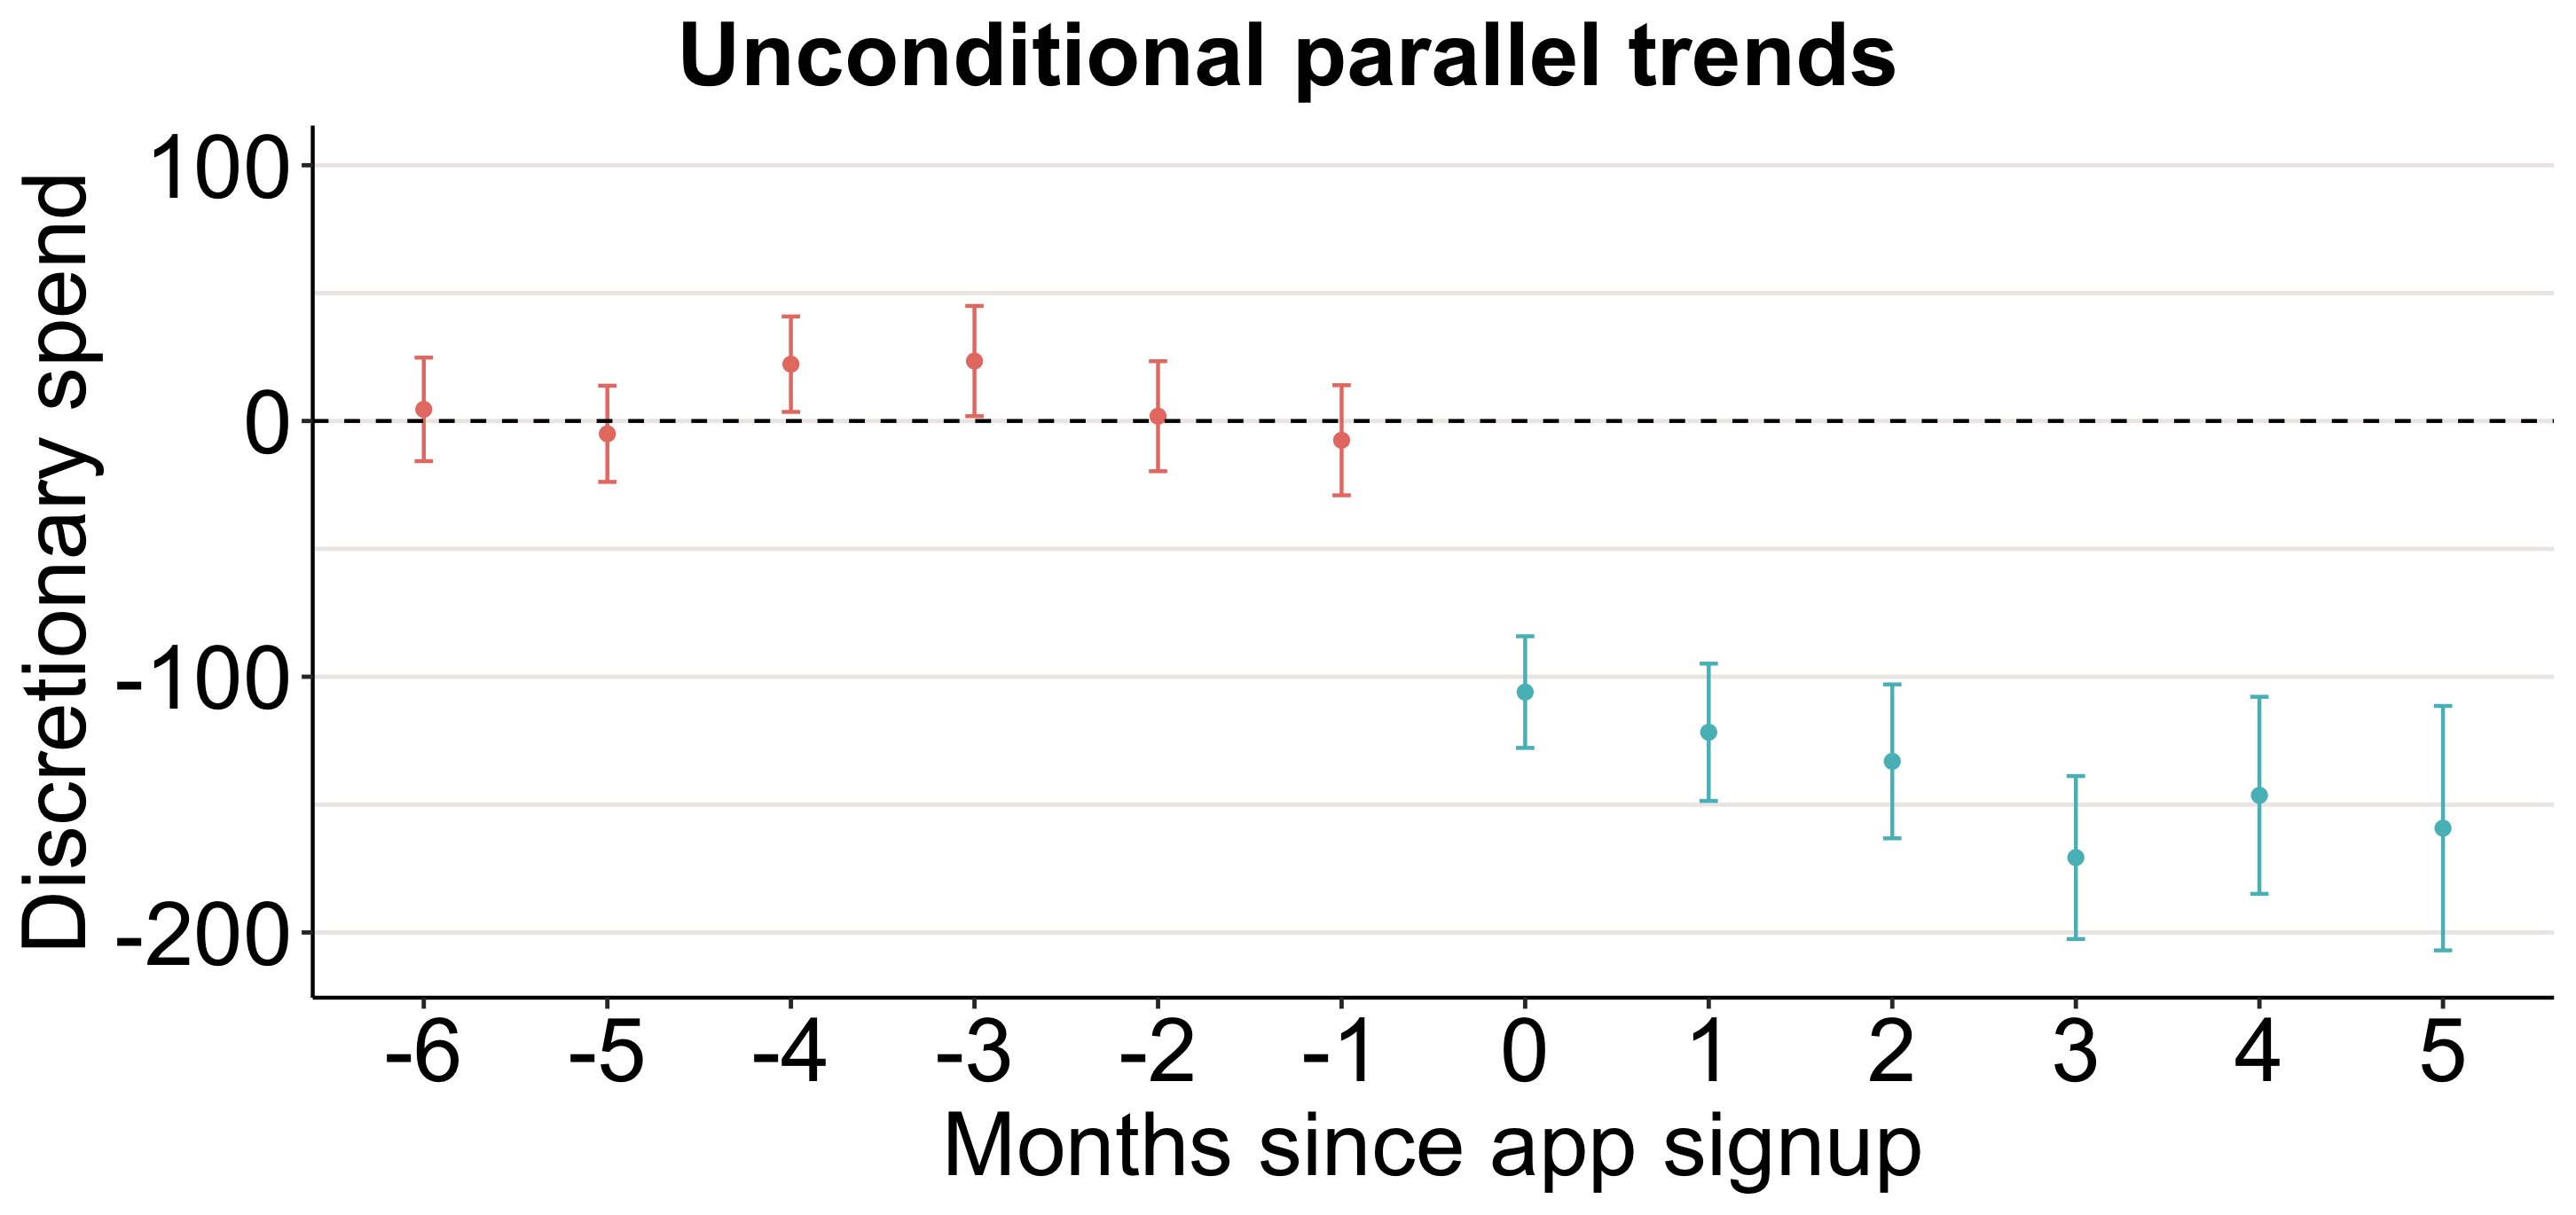
\includegraphics[width=.49\textwidth]{\figdir/dspend_uncond_es.png}
    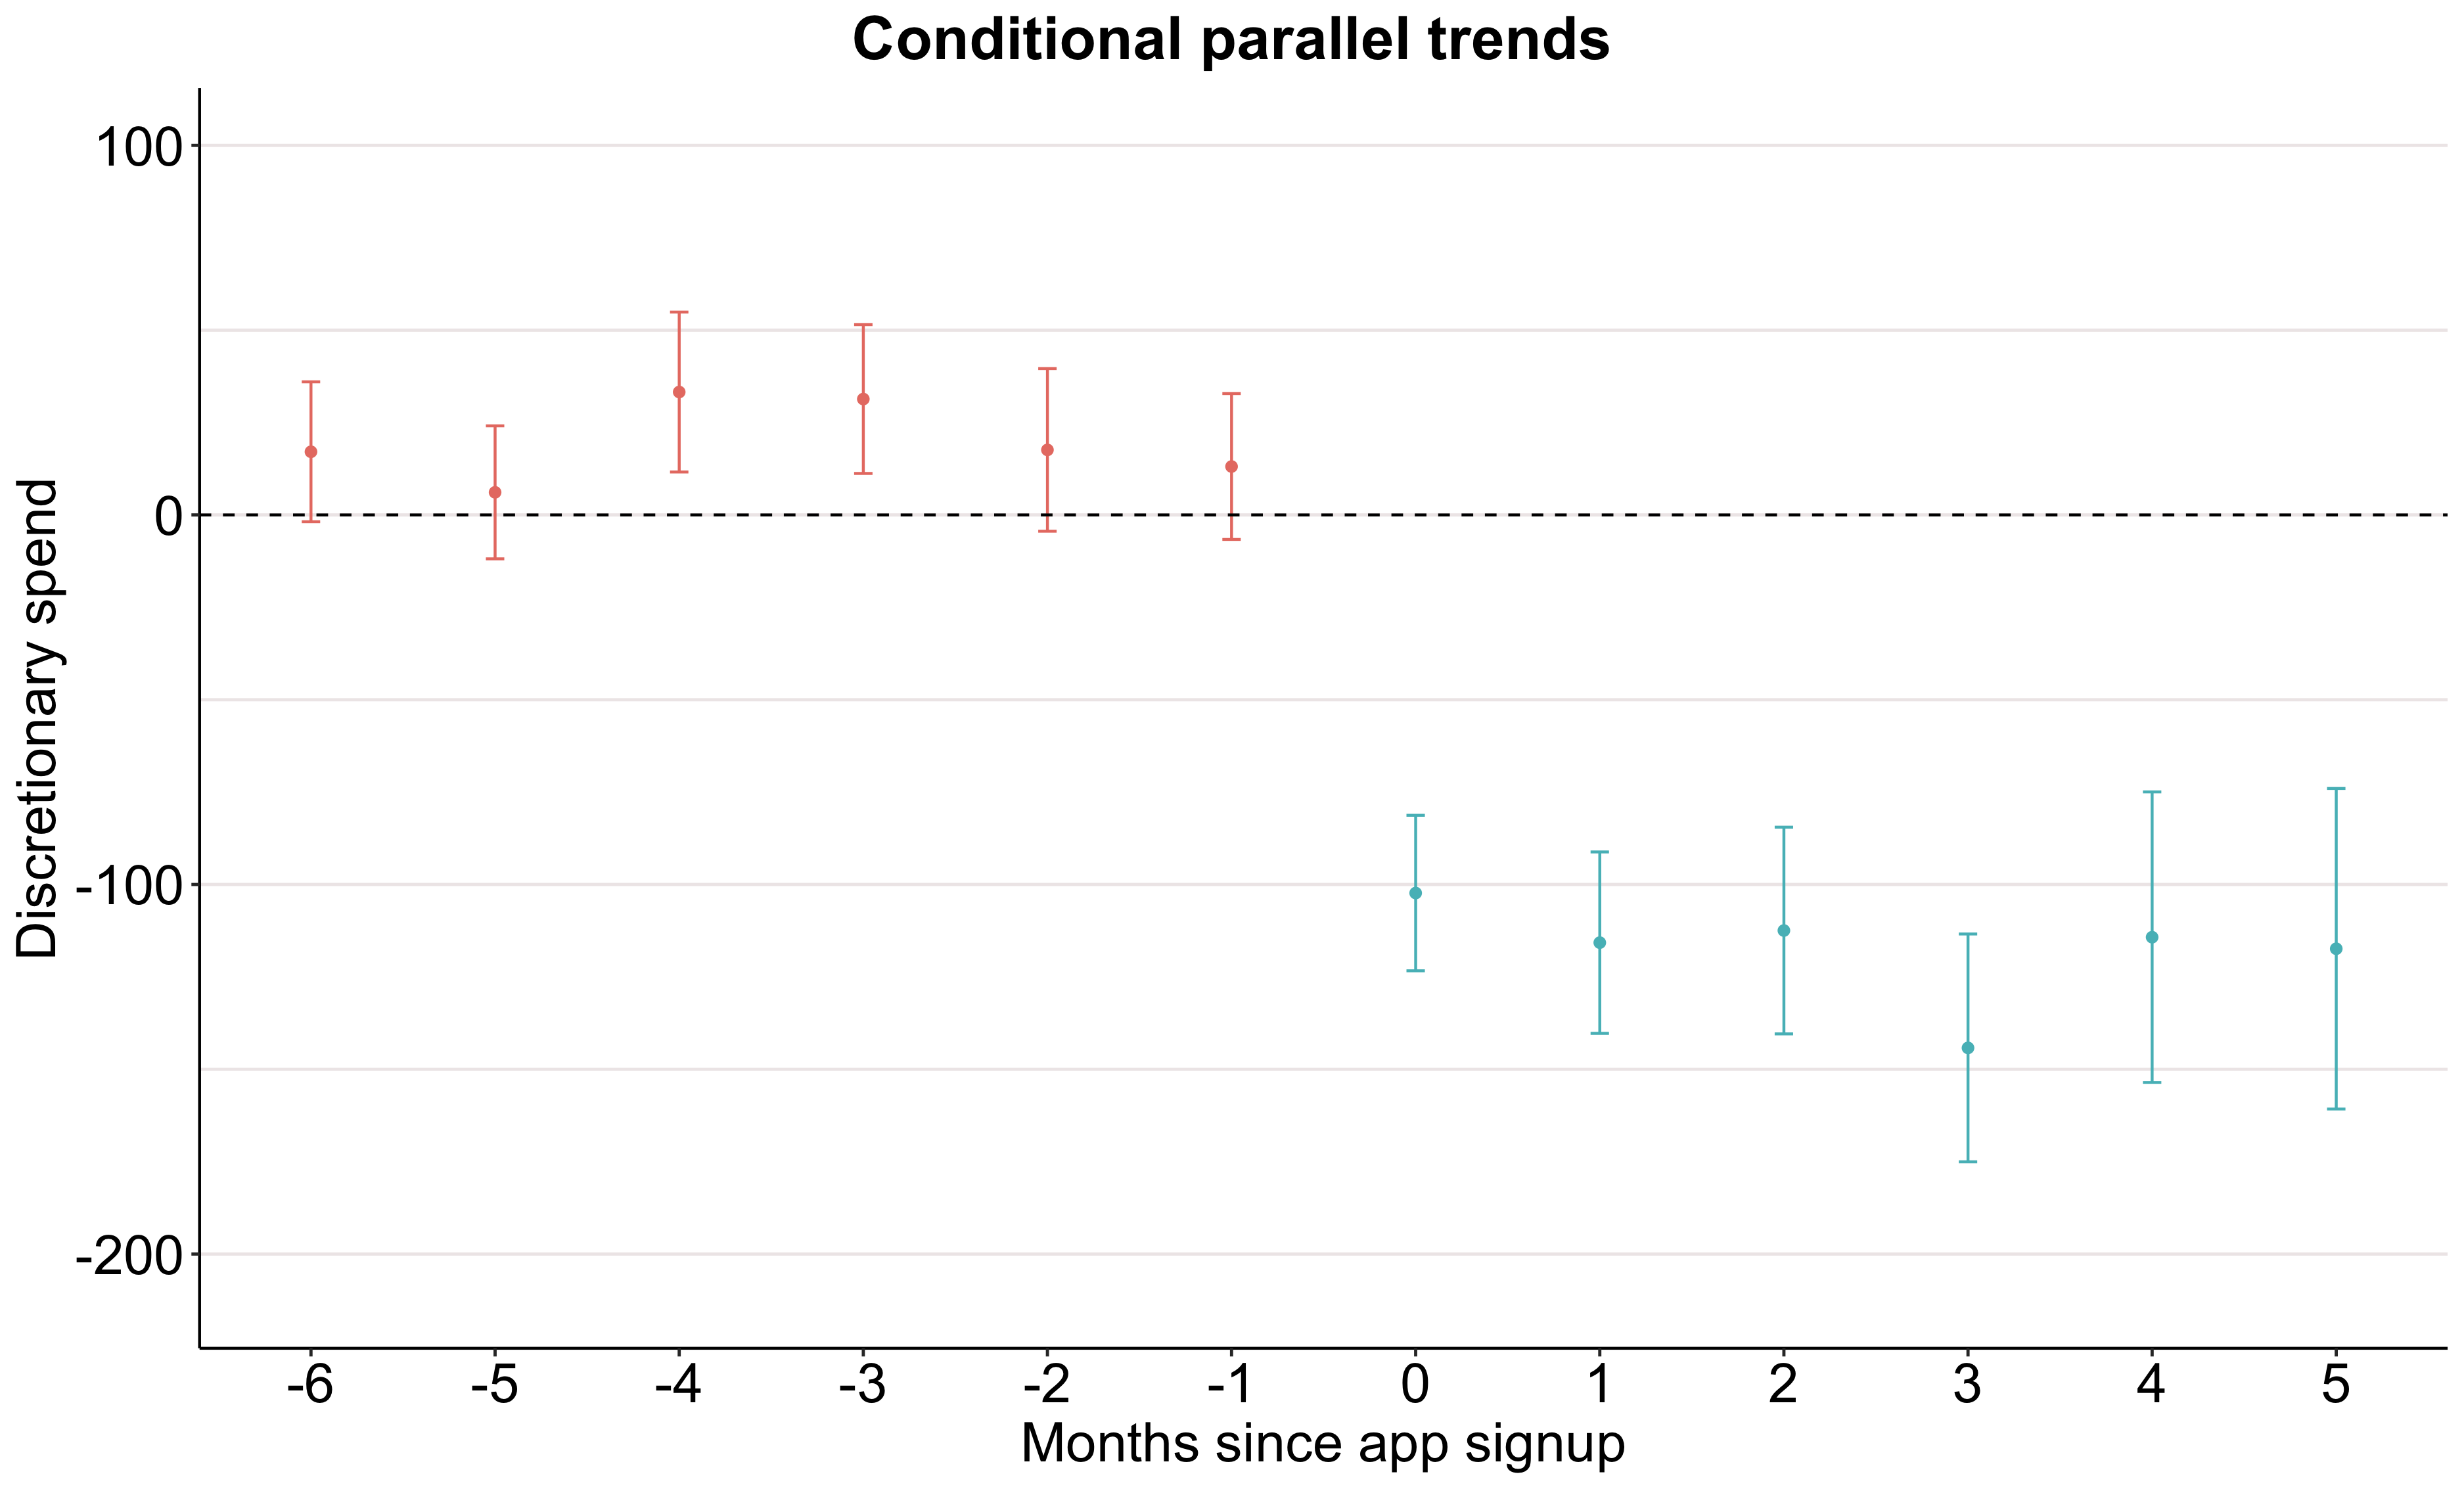
\includegraphics[width=.49\textwidth]{\figdir/dspend_cond_es.png}
    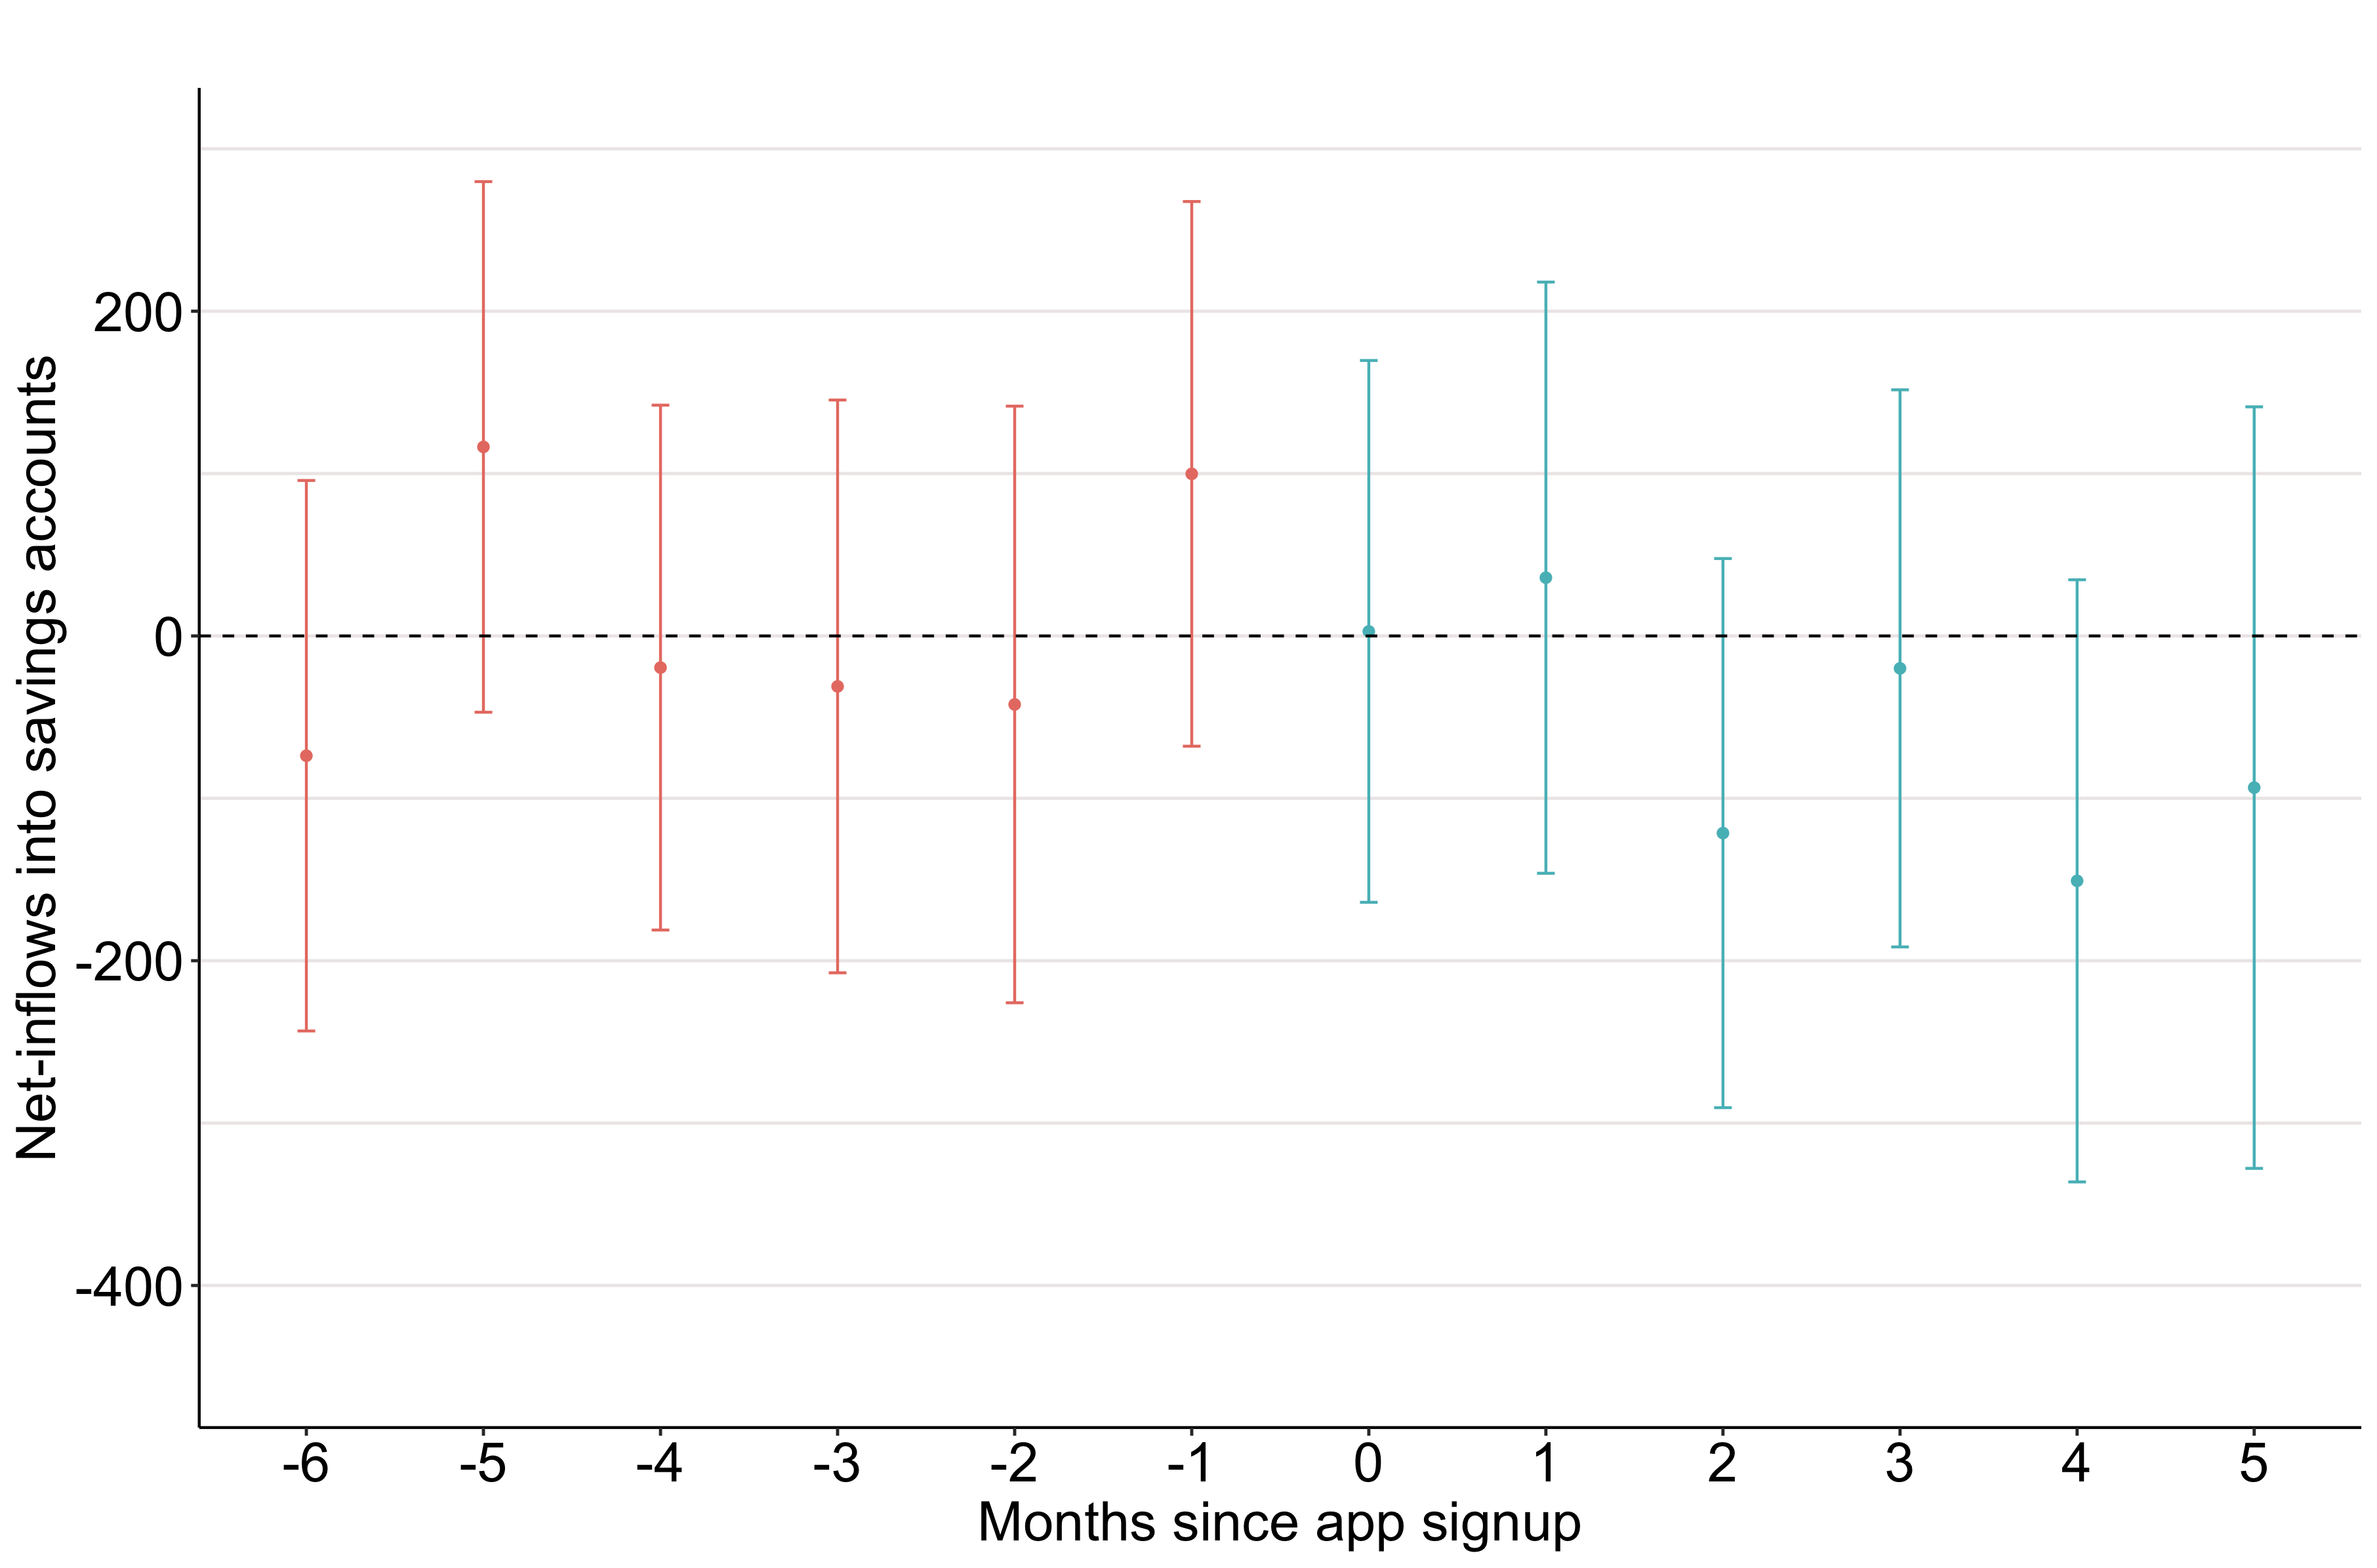
\includegraphics[width=.49\textwidth]{\figdir/netflows_uncond_es.png}
    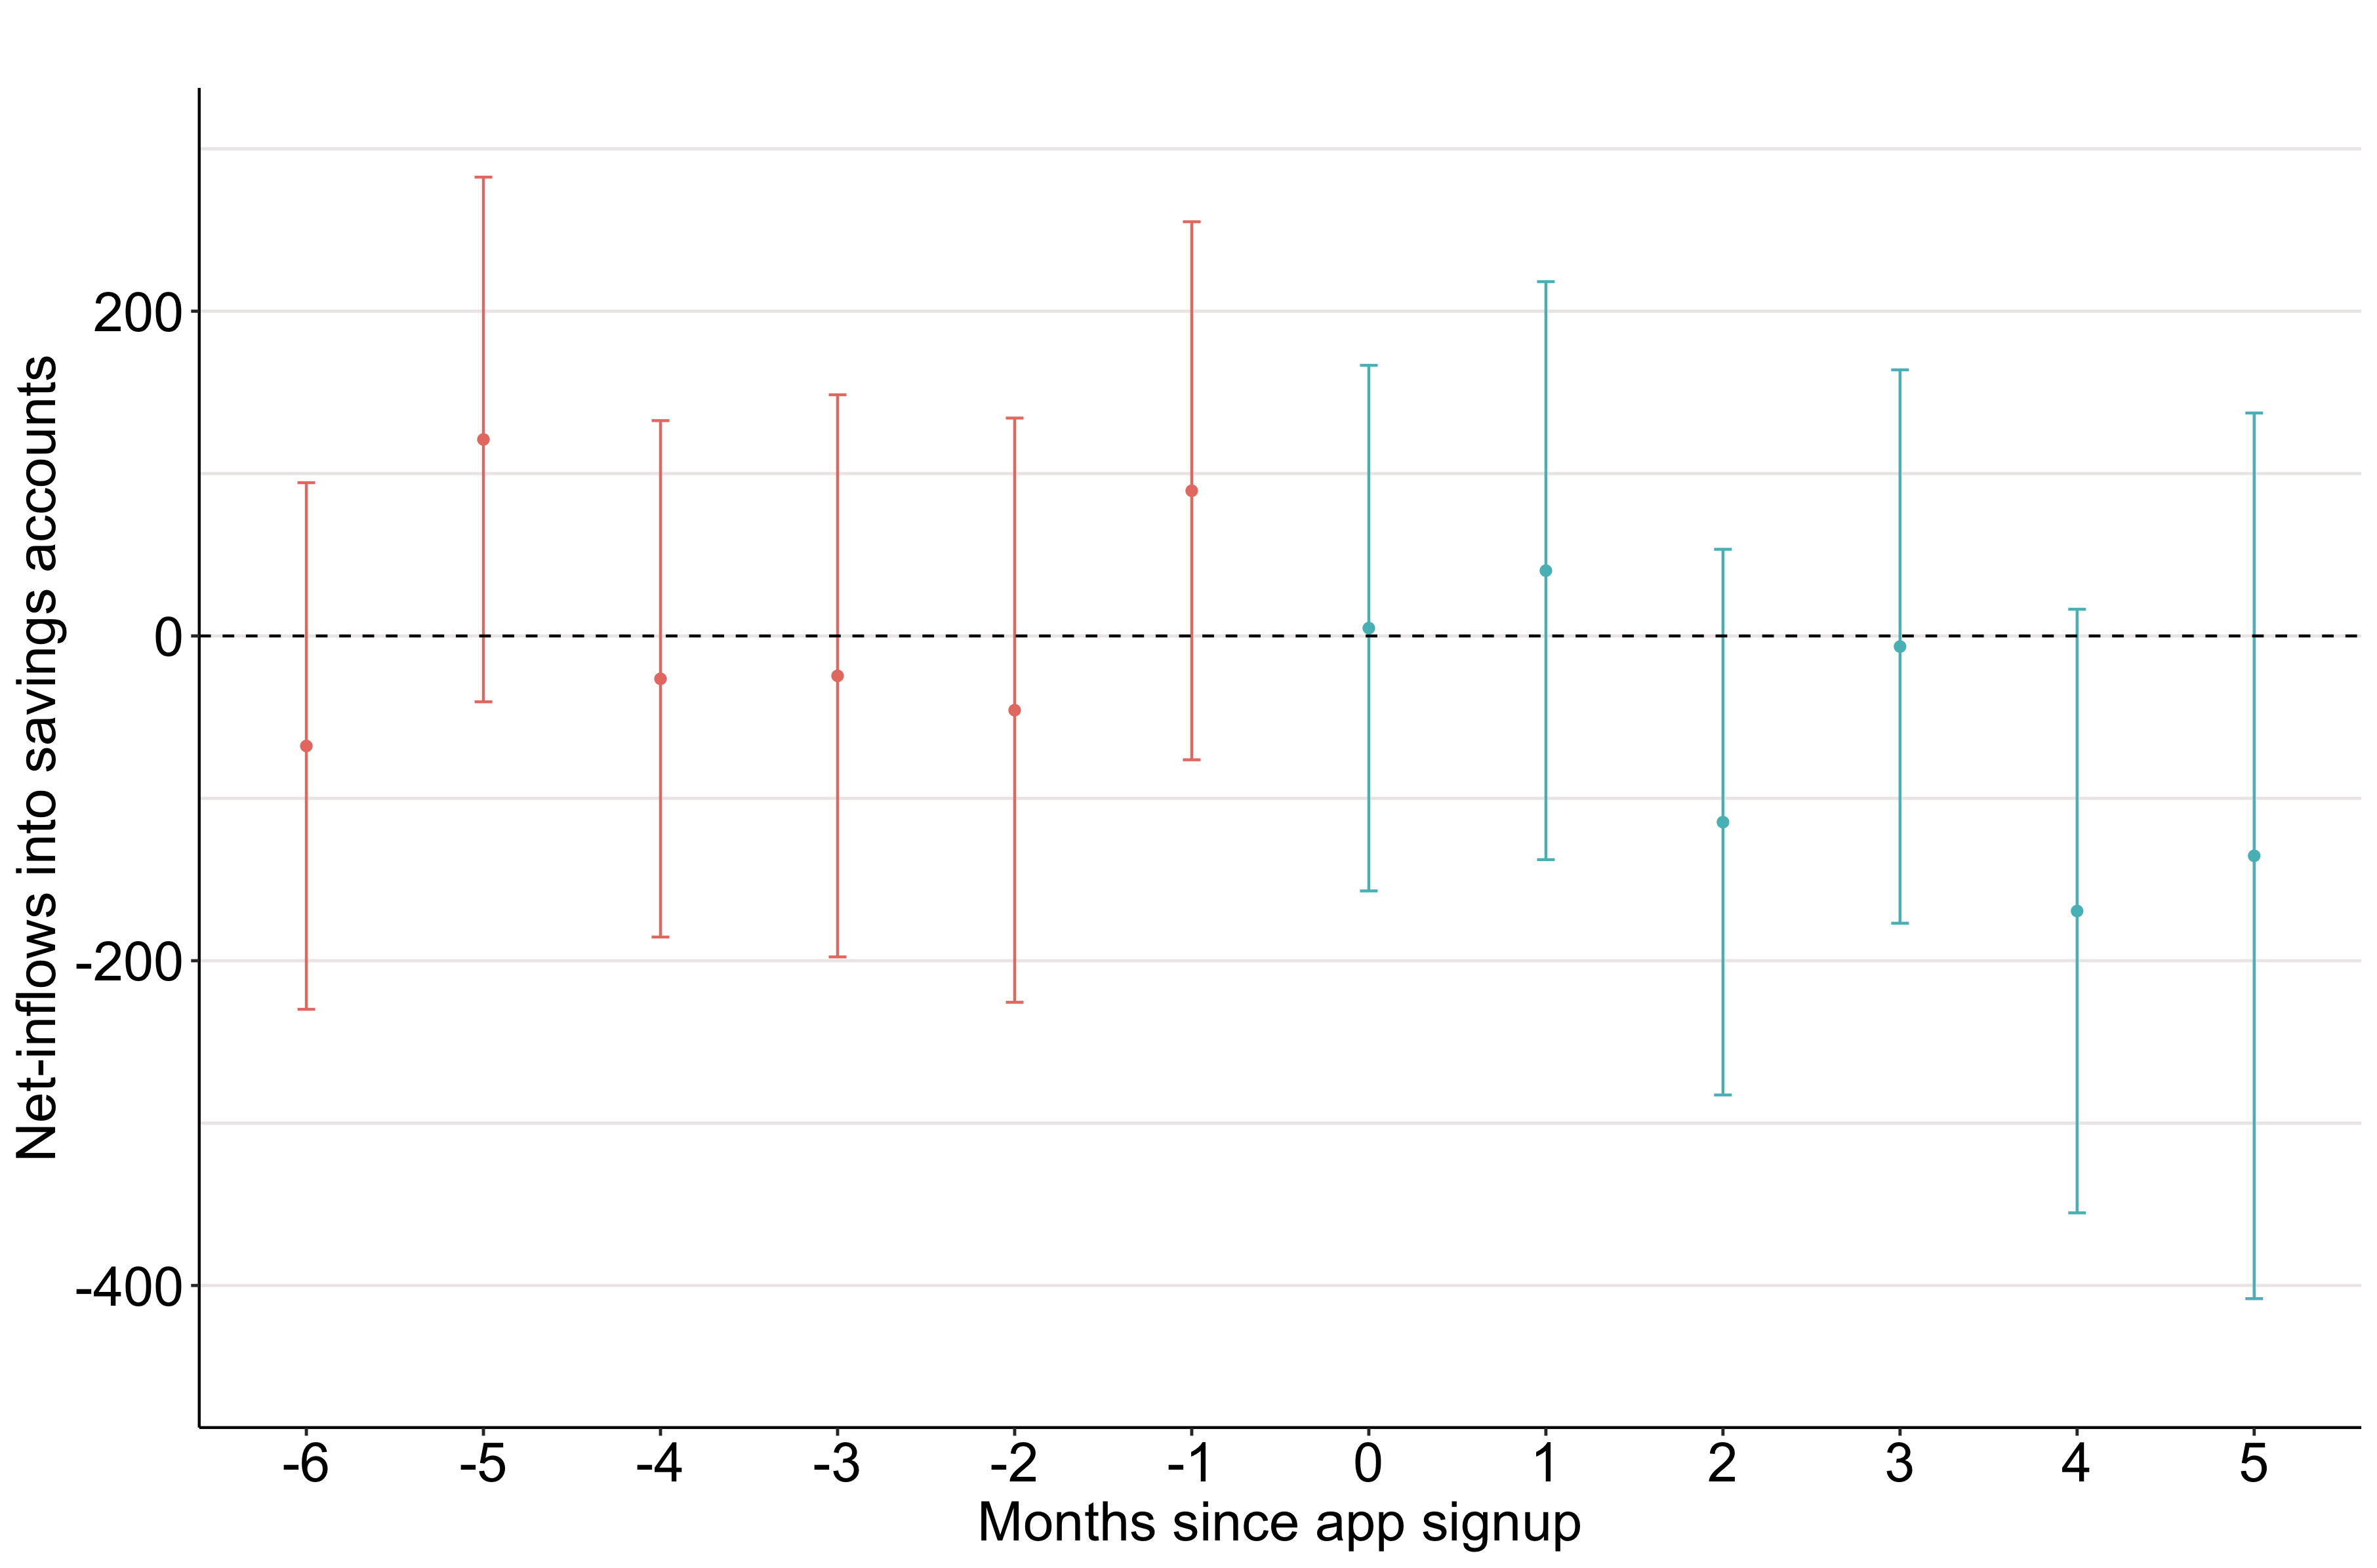
\includegraphics[width=.49\textwidth]{\figdir/netflows_cond_es.png}
    \fignote{\textwidth}{The effect of app use on monthly discretionary
        spending (top row) and monthly net-inflows into savings accounts
        (bottom row) under the unconditional (left column) and conditional
        (right column) parallel trends assumption. Point estimates represent
        group-time average treatment effects aggregated to periods since
        treatment exposure, as defined in Section~\ref{sub:estimation}. Red
        lines represent point estimates and uniform 95\% confidence bands for
        pre-treatment periods allowing for clustering at the user level. If the
        null hypothesis that parallel trends hold in all periods is correct,
        these should be equal to zero. Blue lines provide similar information
    for post-treatment periods.}
\end{figure}


\subsection{Intensive and extensive margins}%
\label{sub:intensive_and_extensive_margins}

\begin{itemize}

    \item Figure~\ref{fig:int_ext_results} shows the effect of app use on
        monthly discretionary spend (top row) and net-inflows into savings
        accounts (bottom row) disaggregated into the effect on the extensive
        (left column) and intensive (right column) margins. For discretionary
        spend, the extensive margin is the number of discretionary transactions
        per month, and the intensive margin is the average value of a
        discretionary spend transaction. For net-inflows into savings accounts,
        the extensive margin is the probability that net-inflows are positive
        in a given month, and the intensive margin is the value of net-inflows
        if net-inflows are positive.

    \item We can see that the reduction of discretionary spend seen in
        Figure~\ref{fig:main_results} is driven by changes on the extensive
        margin: users make about five fewer discretionary purchases once they
        start using the app, while the average amount of each purchase stays
        unchanged (and actually increases slightly over time). The mean value
        of a discretionary spend tranaction in our data is about \pounds25, so
        that five transactions account for the effect shown in the main
        results.

    \item As in the aggregated effects above, app use has no effect on savings
        behaviour.

\end{itemize}

\begin{figure}[H]
    \centering
    \caption{Intensive and extensive margins}%
    \label{fig:int_ext_results}
    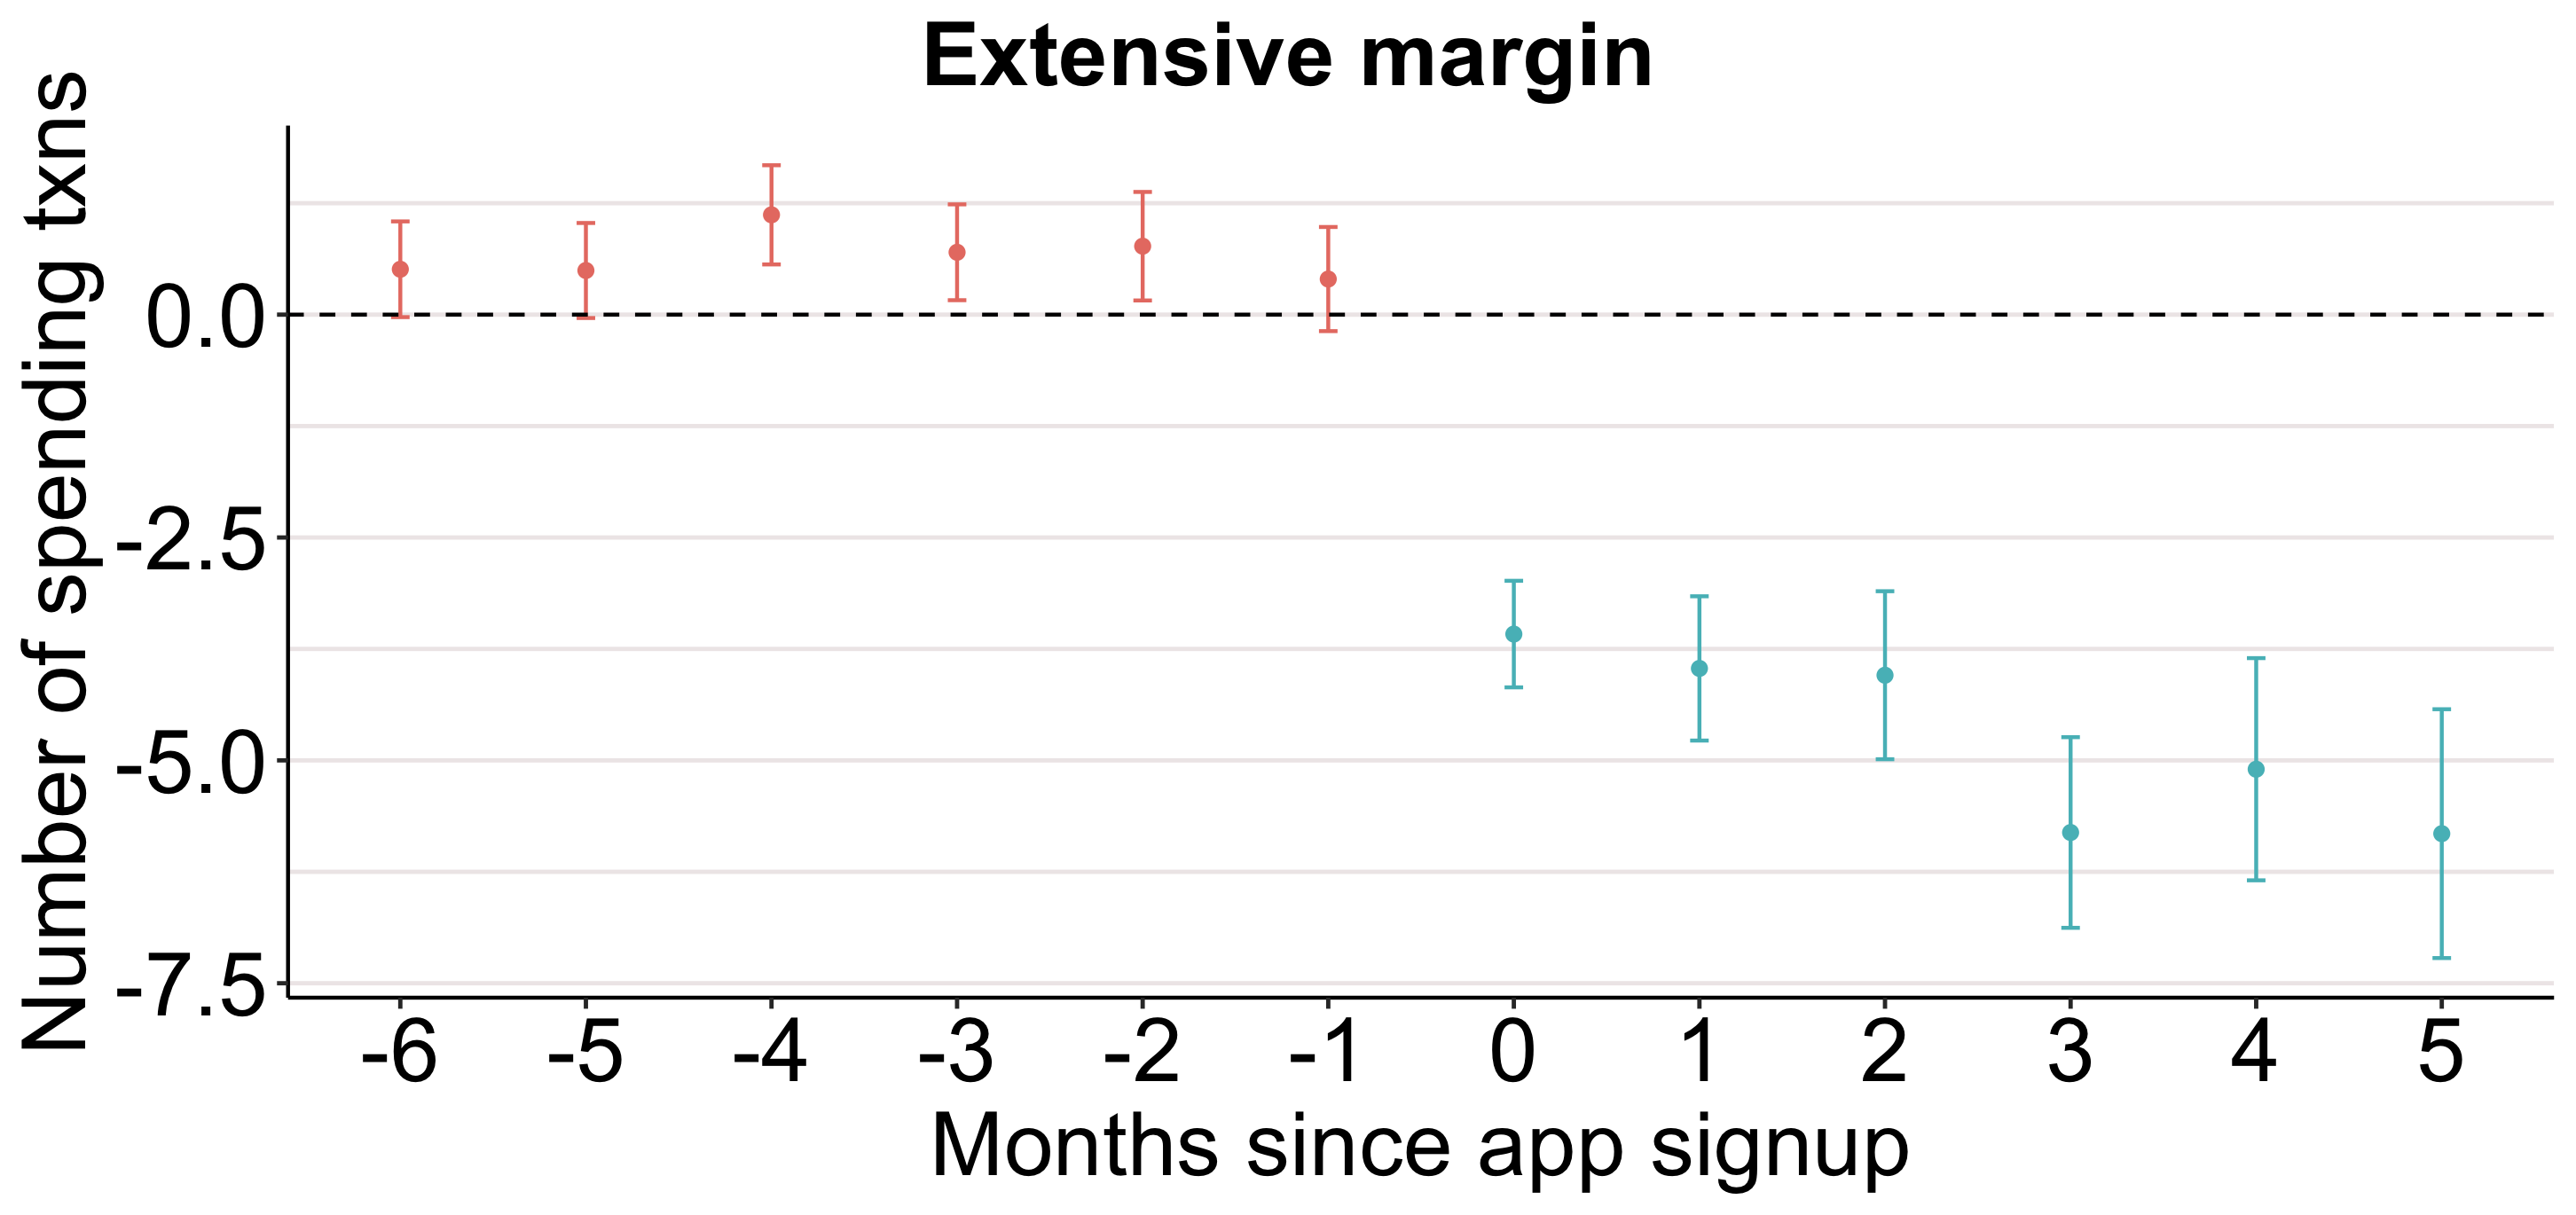
\includegraphics[width=.49\textwidth]{\figdir/dspend_extens_es.png}
    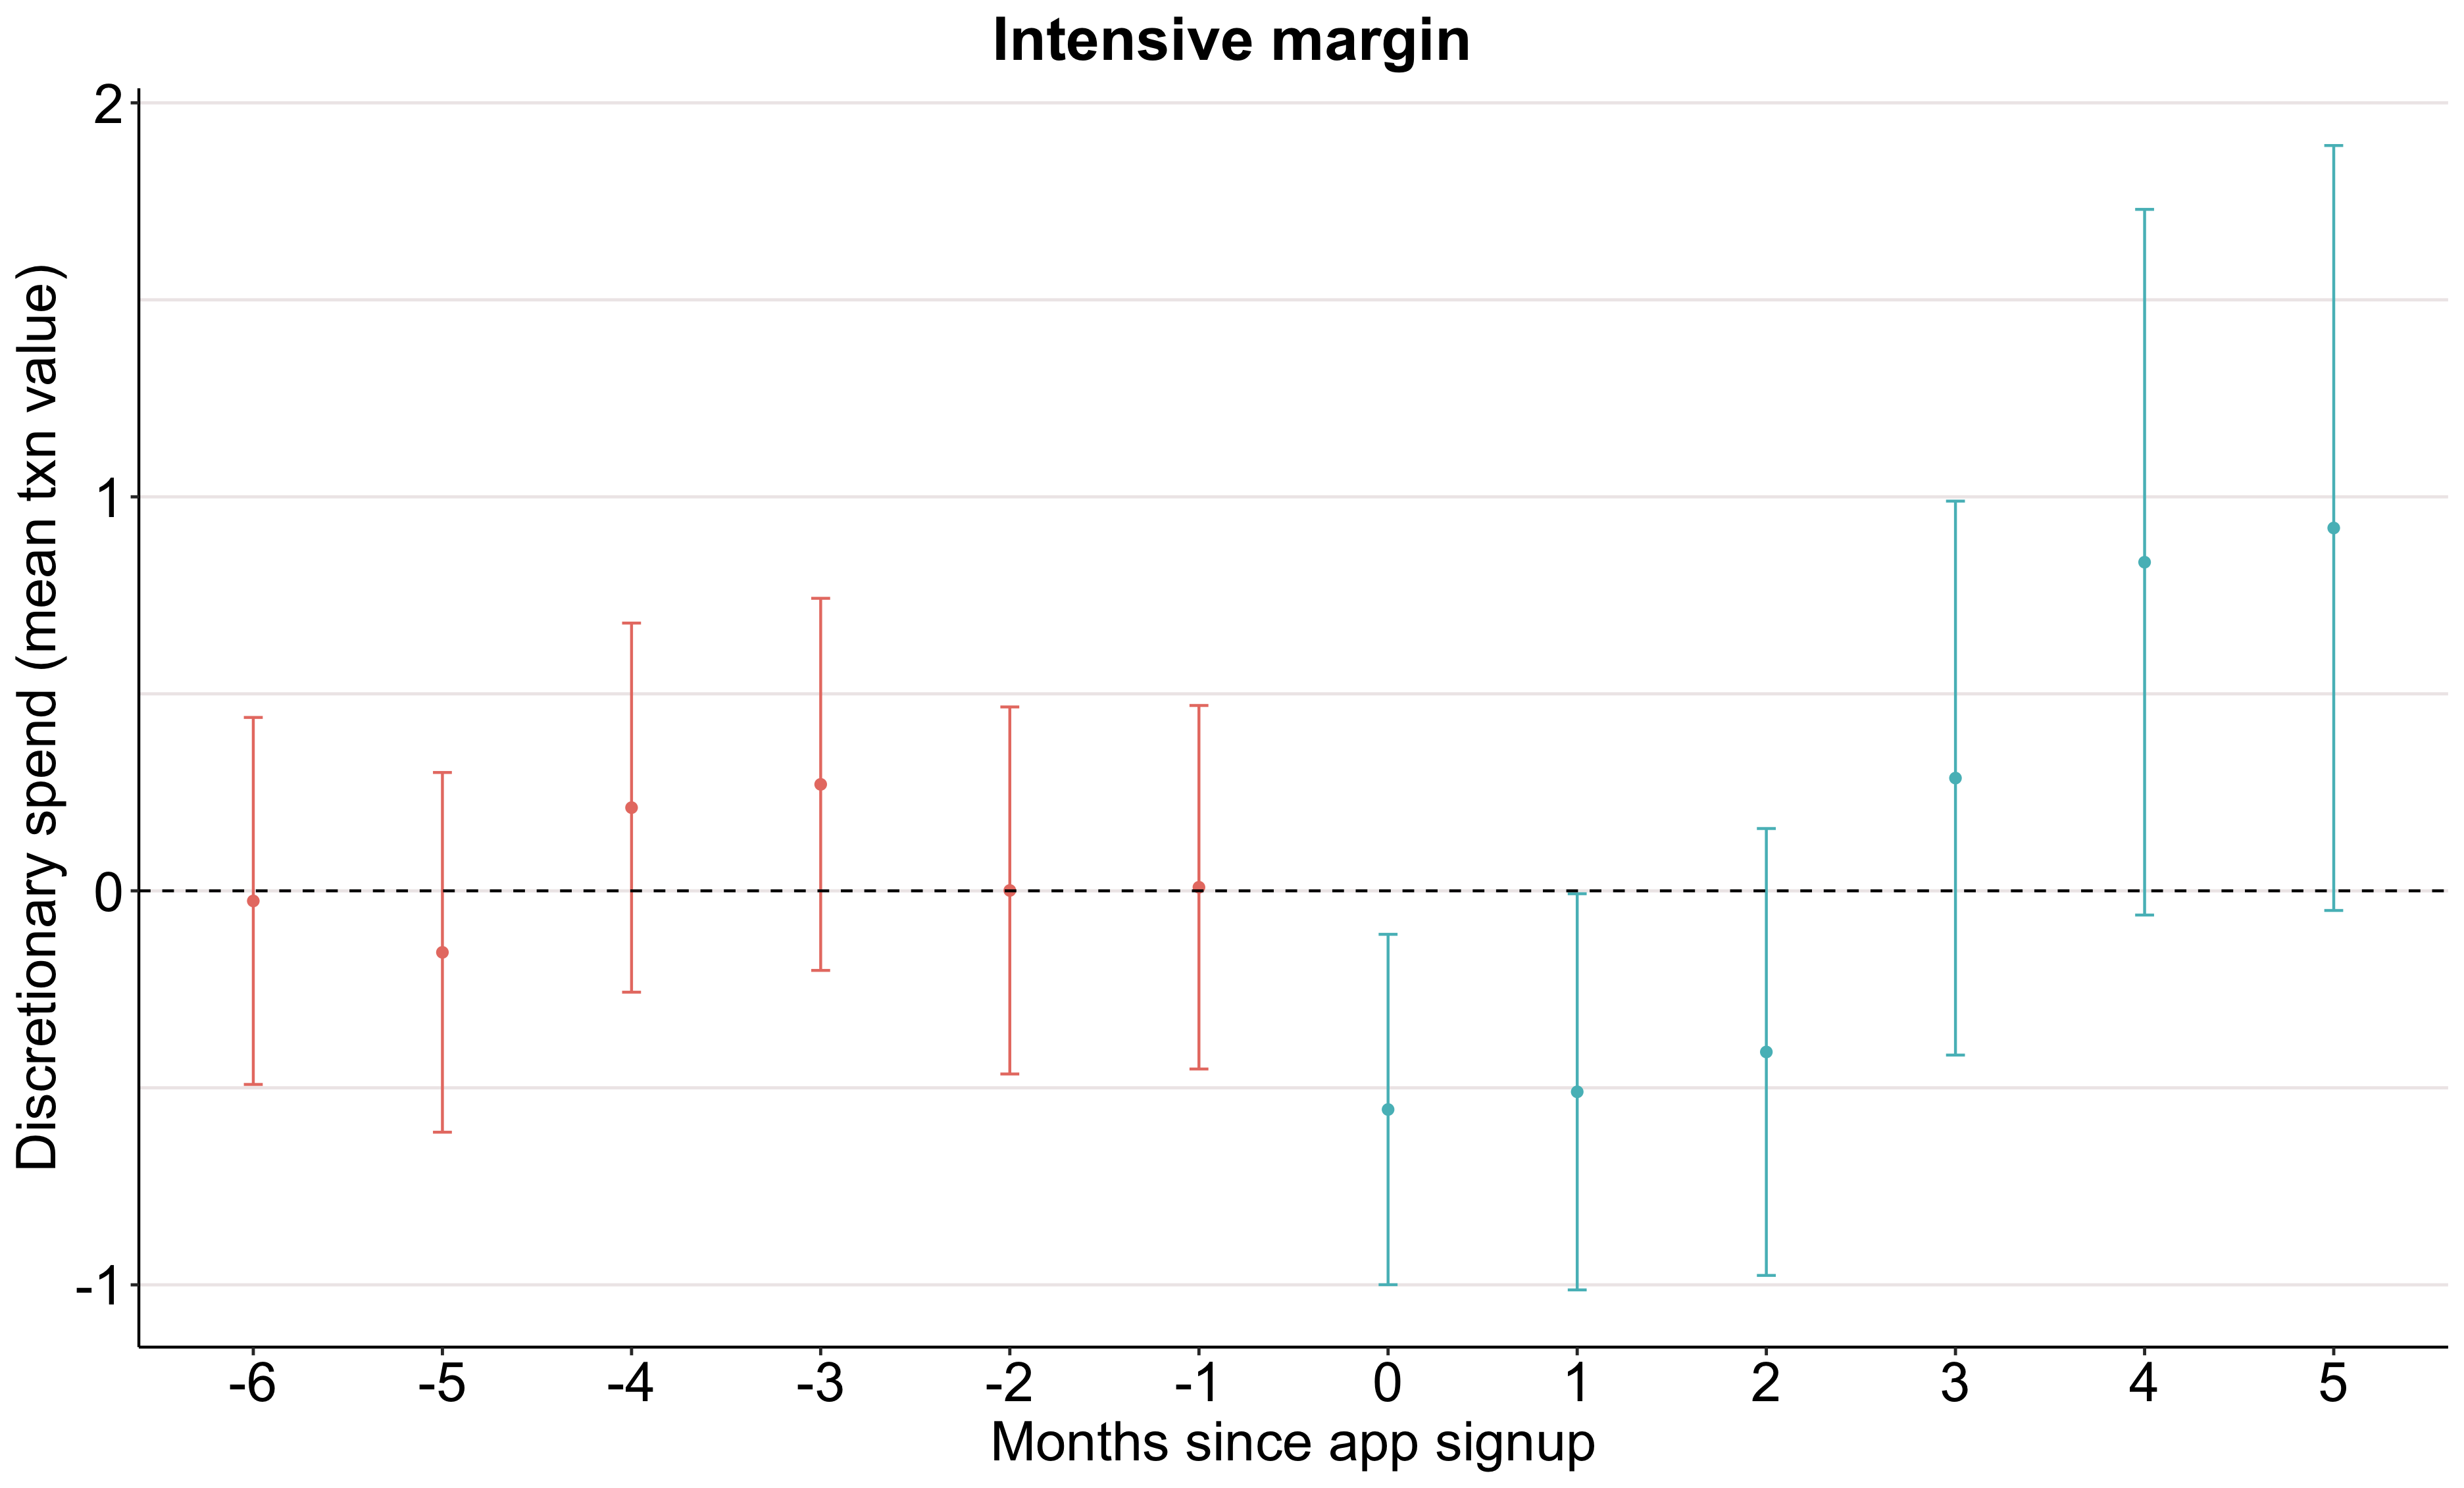
\includegraphics[width=.49\textwidth]{\figdir/dspend_intens_es.png}
    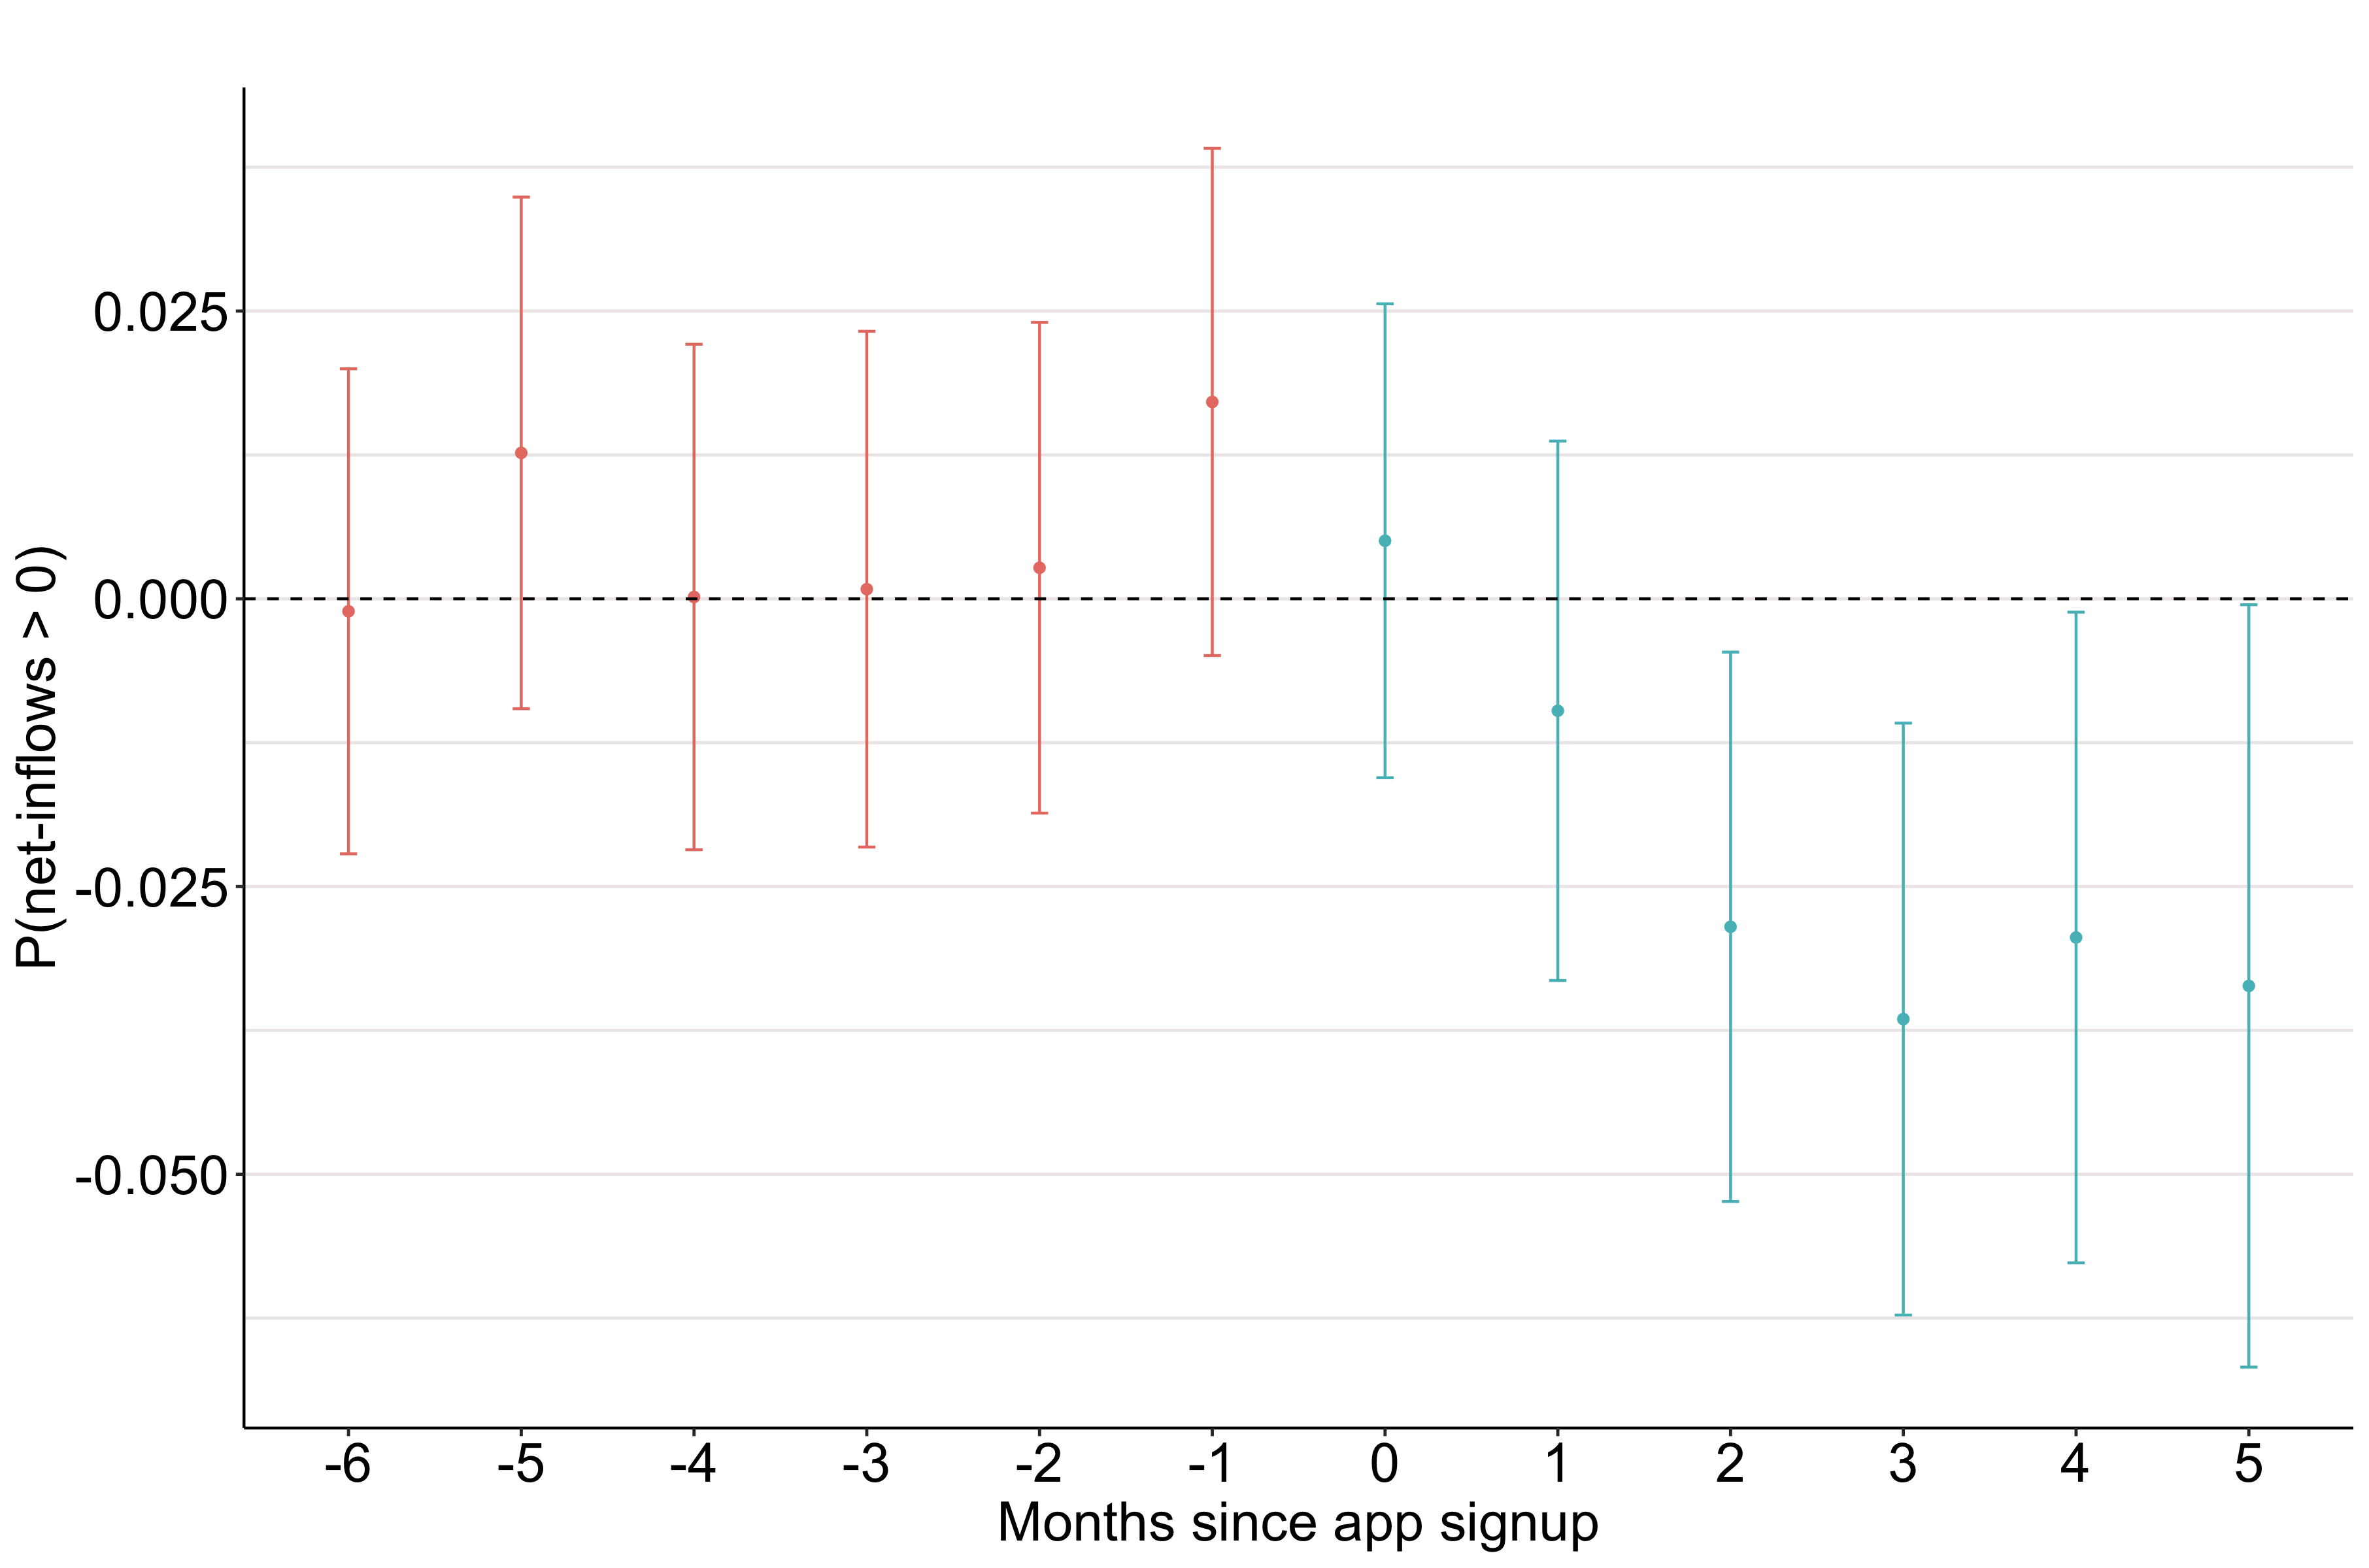
\includegraphics[width=.49\textwidth]{\figdir/netflows_extens_es.png}
    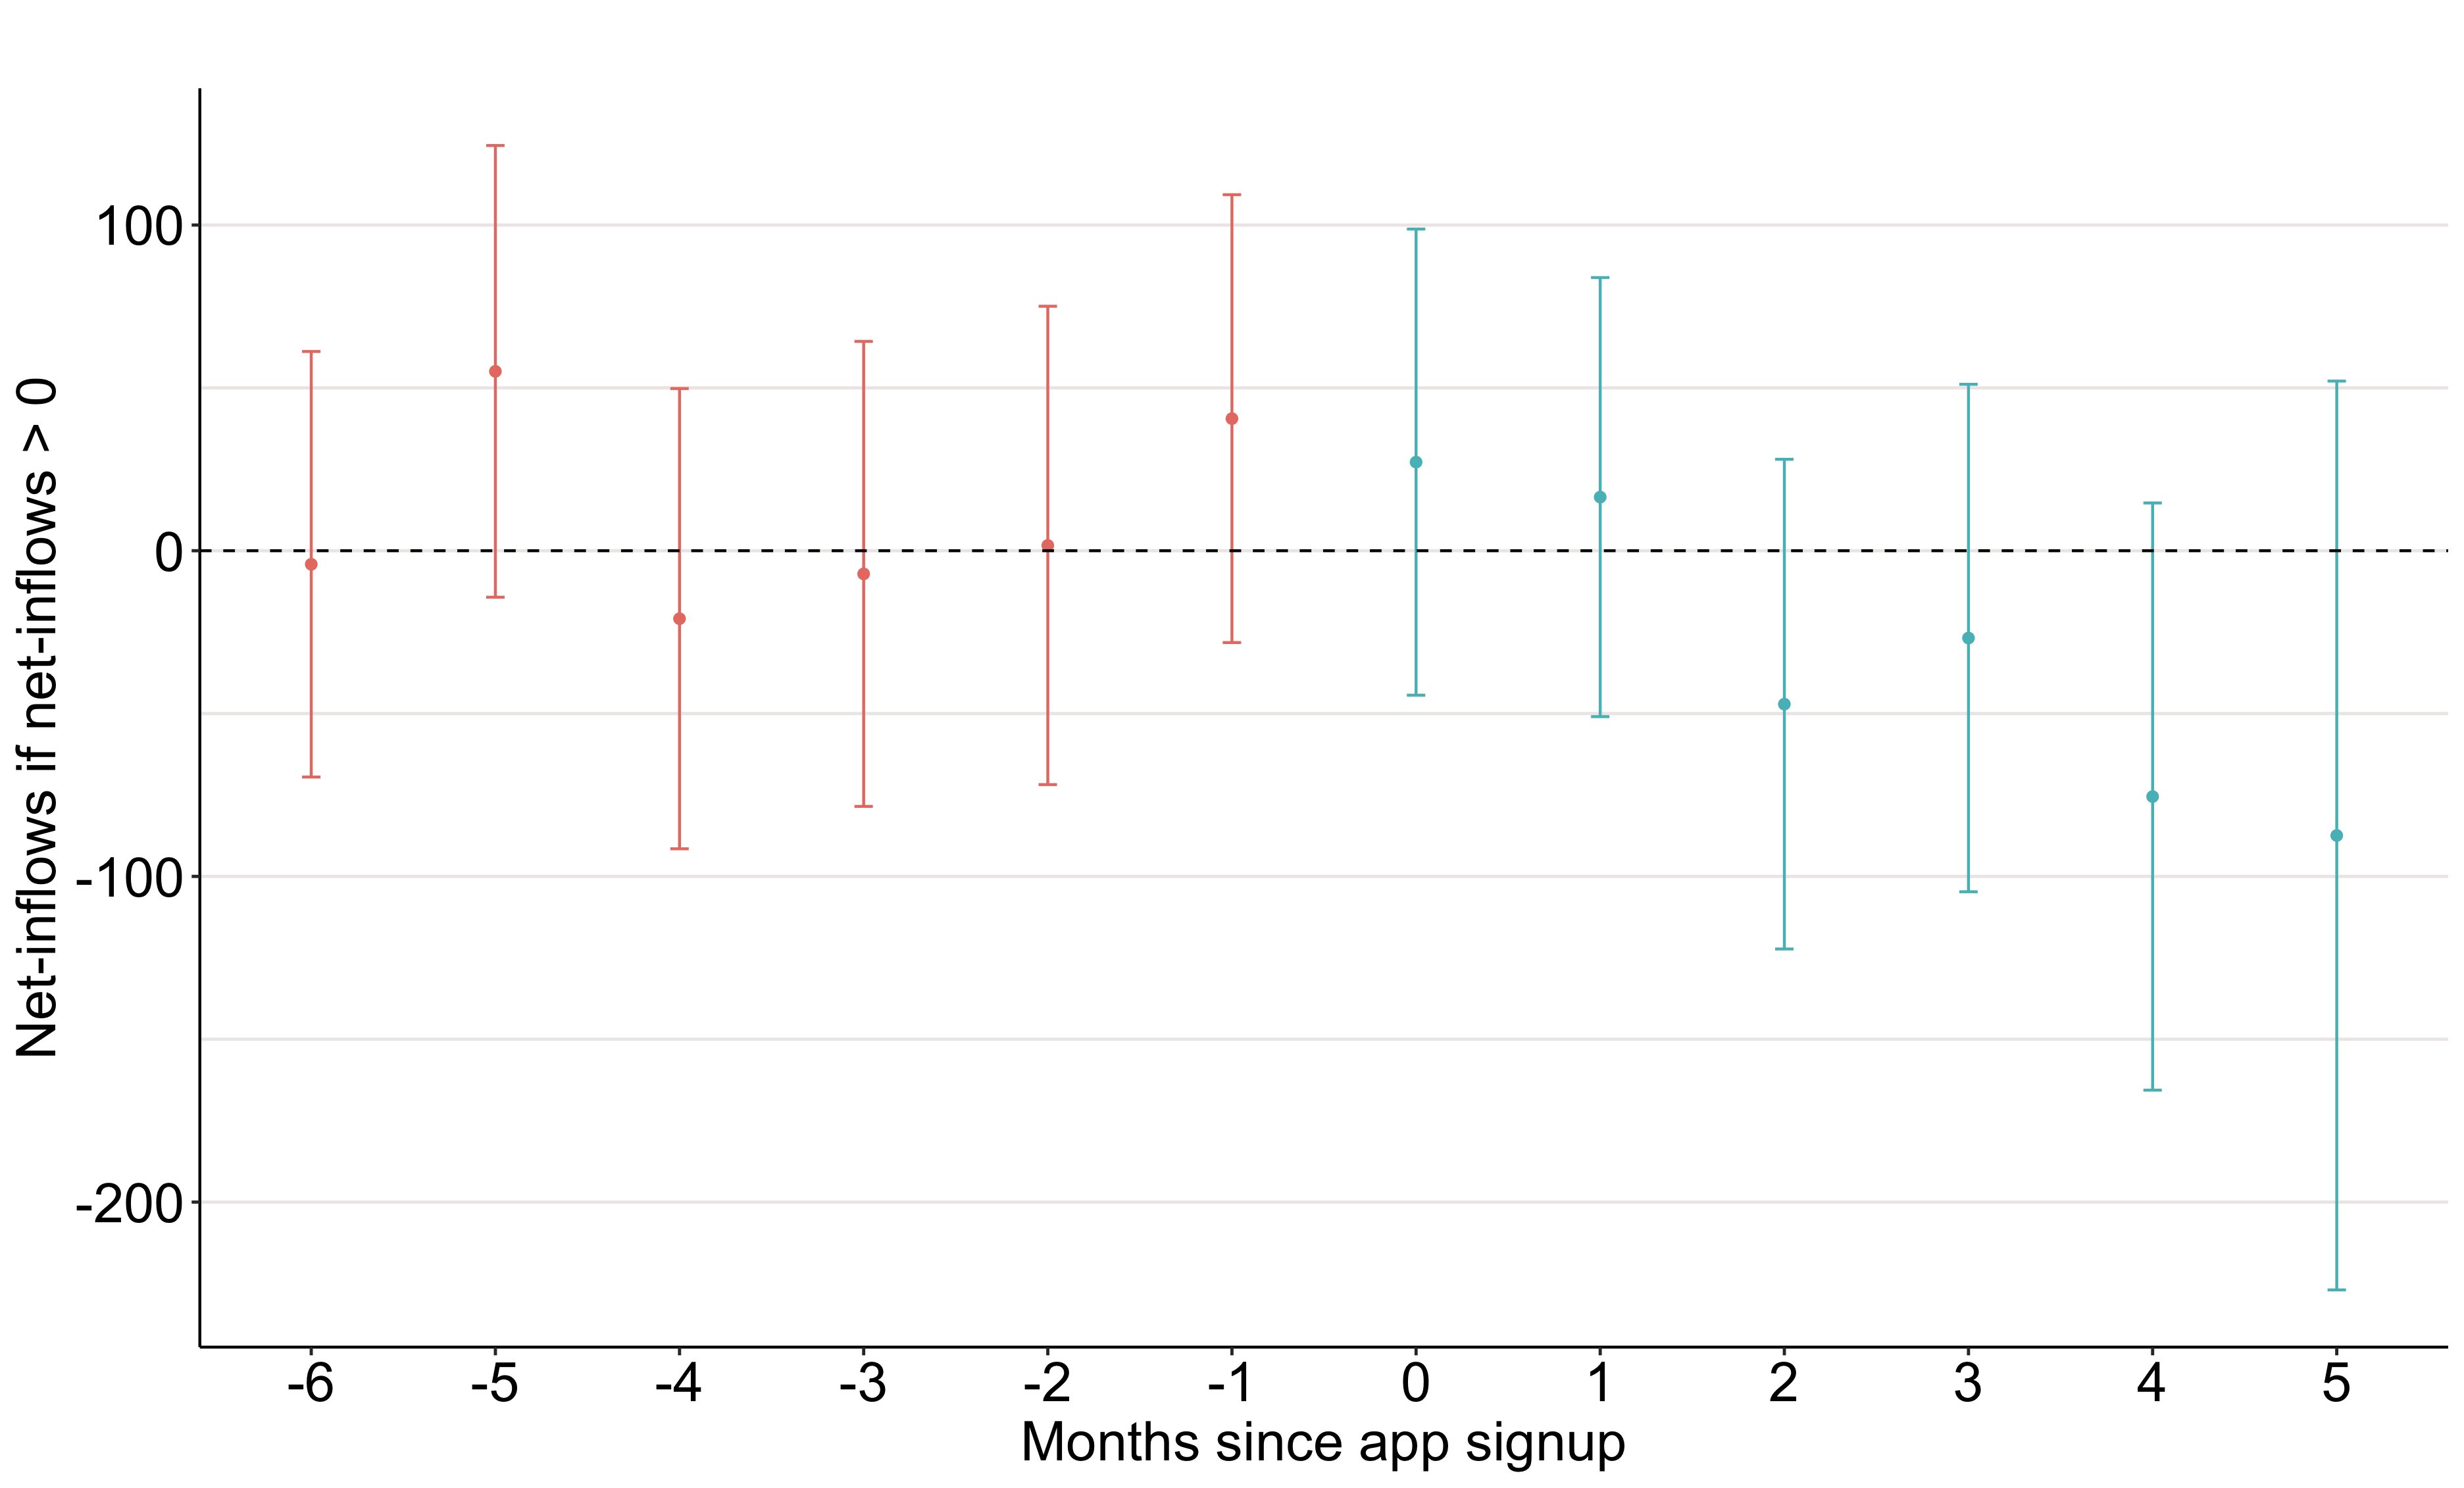
\includegraphics[width=.49\textwidth]{\figdir/netflows_intens_es.png}
    \fignote{\textwidth}{The effect of app use on monthly discretionary spend
        (top row) and net-inflows into savings accounts (bottom row)
        disaggregated into the effect on the extensive (left column) and
        intensive (right column) margins. For discretionary spend, the
        extensive margin is the number of discretionary transactions per month,
        and the intensive margin is the average value of a discretionary spend
        transaction. For net-inflows into savings accounts, the extensive
        margin is the probability that net-inflows are positive in a given
        month, and the intensive margin is the value of net-inflows if
        net-inflows are positive. Point estimates represent
        group-time average treatment effects aggregated to periods since
        treatment exposure, as defined in Section~\ref{sub:estimation}. Red
        lines represent point estimates and uniform 95\% confidence bands for
        pre-treatment periods allowing for clustering at the user level. If the
        null hypothesis that parallel trends hold in all periods is correct,
        these should be equal to zero. Blue lines provide similar information
    for post-treatment periods.}
\end{figure}


